\documentclass{article}

\usepackage[utf8]{inputenc}

\usepackage{amsmath}

\usepackage{scrextend}

\usepackage{geometry}
\geometry{
	a4paper,
	total={170mm,257mm},
	left=20mm,
	top=20mm,
}

\usepackage{graphicx}
\usepackage[portuguese]{babel}
\usepackage{subfig}


\usepackage{listings}
\usepackage{xcolor}

\definecolor{codegreen}{rgb}{0,0.6,0}
\definecolor{codegray}{rgb}{0.5,0.5,0.5}
\definecolor{codepurple}{rgb}{0.58,0,0.82}
\definecolor{backcolour}{rgb}{0.95,0.95,0.92}

\lstdefinestyle{mystyle}{
	backgroundcolor=\color{backcolour},   
	commentstyle=\color{codegreen},
	keywordstyle=\color{magenta},
	numberstyle=\tiny\color{codegray},
	stringstyle=\color{codepurple},
	basicstyle=\ttfamily\footnotesize,
	breakatwhitespace=false,         
	breaklines=true,                 
	captionpos=b,                    
	keepspaces=true,                 
	numbers=left,                    
	numbersep=5pt,                  
	showspaces=false,                
	showstringspaces=false,
	showtabs=false,                  
	tabsize=2
}

\lstset{style=mystyle}

%\usepackage{indentfirst}
\setlength{\parindent}{1.5cm}% too much in my eyes delete this
% line and use the default ...


\title{
	Aplicando técnicas de meios-tons por difusão de erro (trabalho 2) \\
	\Large Introdução ao Processamento de Imagem Digital \\
	Randerson A. Lemos (103897)
	2022-1S
}

\date{\vspace{-5ex}}

\begin{document}
  \pagenumbering{gobble}
  \maketitle

%
%%
\section{Introdução}
As técnicas de meios-tons se prestam a quantizar as cores de uma imagem (reduzir a quantidade de cores que possui) enquanto procuram manter a imagem resultante, do ponto de vista da percepção visual, o menos alterada possível. Neste trabalho, foram aplicadas as seguintes técnicas de meios-tons por difusão de erro:

\begin{table*}[h]
	\caption*{Floyd e Steinberg}
	\label{tab:floyd}
	\centering
	\begin{tabular}{|l|l|l|}
		\hline
		& f(x,y) & 7/16 \\ \hline
		3/16 & 5/16   & 1/16 \\ \hline
	\end{tabular}
\end{table*}

\begin{table}[h]
	\caption*{Stevenson e Arce}
	\label{tab:stevenson}
	\centering
	\begin{tabular}{|l|l|l|l|l|l|l|}
		\hline
		&        &        & f(x,y) &        & 32/200 &        \\ \hline
		12/200 &        & 26/200 &        & 30/200 &        & 16/200 \\ \hline
		& 12/200 &        & 26/200 &        & 12/200 &        \\ \hline
		5/200  &        & 12/200 &        & 12/200 &        & 5/200  \\ \hline
	\end{tabular}
\end{table}

\begin{table}[h]
	\caption*{Burkes}
	\label{tab:burkers}
	\centering
	\begin{tabular}{|l|l|l|l|l|}
		\hline
		&      & f(x,y) & 8/32 & 4/32 \\ \hline
		2/32 & 4/32 & 8/32   & 4/32 & 2/32 \\ \hline
	\end{tabular}
\end{table}

\begin{table}[!h]
	\caption*{Sierra}
	\label{tab:sierra}
	\centering
	\begin{tabular}{|l|l|l|l|l|}
		\hline
		&      & f(x,y) & 5/32 & 3/32 \\ \hline
		2/32 & 4/32 & 5/32   & 4/32 & 2/32 \\ \hline
		& 2/32 & 3/32   & 2/32 &      \\ \hline
	\end{tabular}
\end{table}

\begin{table}[!h]
	\caption*{Stucki}
	\label{tab:stucki}
	\centering
	\begin{tabular}{|l|l|l|l|l|}
		\hline
		&      & f(x,y) & 8/42 & 4/32 \\ \hline
		2/42 & 4/42 & 8/42   & 4/42 & 2/42 \\ \hline
		1/42 & 2/42 & 4/42   & 2/42 & 1/42 \\ \hline
	\end{tabular}
\end{table}

\begin{table}[!h]
	\caption*{Javis, Judice e Ninke}
	\label{tab:javis}
	\centering
	\begin{tabular}{|l|l|l|l|l|}
		\hline
		&      & f(x,y) & 7/48 & 5/48 \\ \hline
		3/48 & 5/48 & 7/48   & 5/48 & 3/48 \\ \hline
		1/48 & 3/48 & 5/48   & 3/48 & 1/48 \\ \hline
	\end{tabular}
\end{table}

Detalhes se solução e implementação, assim como de análise e conclusão, serão abordados nas seções subsequentes.

%
%%
\section{Solução}
A solução utiliza a linguagem de programação Python e conta com o auxílio do gerenciador de projetos e pacotes Conda. Assumindo que o usuário tenha o Conda instalado em sua máquina, a configuração do projeto pode ser feita pela execução do comando \lstinline{conda env create -f environment.yml} a partir da pasta do projeto \textbf{trab2}. Esse comando cria o ambiente de trabalho \textbf{mc920-trab2} e instala os seguintes módulos: opencv, numpy, scipy, pandas, matplotlib. Finalizada a configuração do ambiente de trabalho em questão, o usuário deve executar o comando \lstinline{source source.sh}\footnote{O comando que configura o ambiente de trabalho mc920-trab2 precisa ser executado apenas um vez. Assim sendo, depois que este ambiente está configurado, o usuário precisa apenas executar o comando \lstinline{source source.sh}} para carregar as variáveis de ambiente adequadas e, assim, poder usar os programas do projeto dentro do próprio ambiente de trabalho recém configurado. 

Dos arquivos presentes na pasta do projeto \textbf{trab2}, destacam-se as pastas \textbf{png}, \textbf{tex} e o programa \textbf{main.py}. A pasta \textbf{png} contém imagens no formato png que podem ser utilizadas para a aplicação das técnicas de meios-tons por difusão de erro. A pasta \textbf{tex} contém os arquivos Latex deste relatório. O programa \textbf{main.py} contém as implementação das soluções de meios-tons por difusão de erro utilizadas. As informações pertinentes do programa \textbf{main.py} são detalhadas a seguir.

%
\subsection{Main.py}
O programa \textbf{main.py} é responsável pela aplicação de todas as técnicas de meios-tons por difusão de erro consideradas neste trabalho. Para ser executado, esse programa precisa receber o parâmetro de entrada \textbf{imagem\_entrada}:

\begin{itemize}
	\item ao parâmetro \textbf{imagem\_entrada} deve-se fornecer o nome do arquivo da imagem a ser utilizada para aplicação das técnicas de meios-tons por difusão de erro selecionadas.
\end{itemize}
	
\noindent

O programa \textbf{main.py} disponibiliza todas as imagens resultantes da aplicação das técnicas de meios-tons em duas versões: uma versão preto e branco e outra versão colorida. Todas essas imagens são salvas dentro da pasta \textbf{out} localizada dentro da pasta do projeto \textbf{trab2}. Há também uma imagem de controle, na qualquer se aplicou um técnica de meio-tom rudimentar, isto é, apenas considerando o limiar de 128 e não utilizando a difusão de erro. Esta imagem também está salva na pasta \textbf{trab2}.

Um exemplo de como executar o programa \textbf{main.py} utilizando os recursos contidos dentro do próprio projeto é: \lstinline{python3 main.py -imagem_entrada=png/baboon.png}.

Sobre a direção de varredura para aplicação das técnicas de meios-tons optou-se por seguir com a direção que percorre a imagem da esquerda para a direita e de cima para baixo como ilustrado em Imagem \ref{fig:direcao_varredura}.

\begin{figure}[htp]%
	\centering
	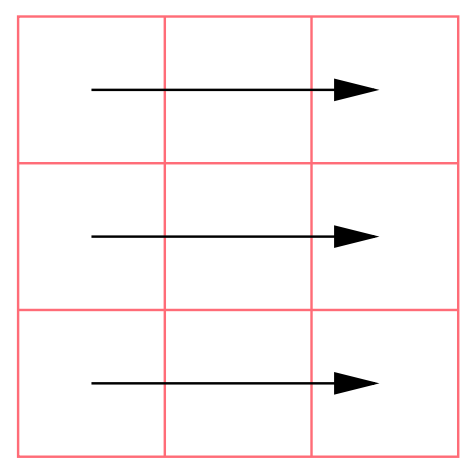
\includegraphics[width=5cm]{./varredura.png} %
	\caption{Direção de varredura considerada para aplicação das técnicas de meios-tons (fonte: imagem extraida do documento pdf com as orientações deste trabalho).}%
	\label{fig:direcao_varredura}%
\end{figure}

Essa opção de varredura foi considera porque a aparência visual das imagens resultantes se mostrou satisfatório, não havendo padrões estranhos que causassem desconforto ao olhar do observador.

Um dos destaques das implementações realizadas é a classe \textbf{Mask}. Essa classe ficou responsável pelo encapsulamento da lógica de recuperação dos pesos das mascaras das técnicas de meios-tons por difusão de erro bem como das posições nas quais estes pesos deveriam ser aplicados na imagem original. Dessa maneira, para o usuário, só ficou necessário passar a matriz da mascara da técnica de meio-tom em questão e a posição de referência do posicionamento na mascara do pixel \textbf{f(x,y)} da imagem original. Essa classe foi implementada como um objeto \textbf{iterador} do Python de modo que a recuperação do pesos bem como da posição de aplicação destes na imagem original era facilmente alcançada dentro de uma estrutura de laço de repetição. Isso tornou bastante conveniente a integração da instancia da classe \textbf{Mask} dentro da função responsável por construir a imagem \textbf{g(x, y)} possuidora dos pixels em meios-tons. A implementação da classe \textbf{Mask} é apresentada a baixo.

\begin{lstlisting}
class Mask:
  def __init__(self, mask):
    self.name = mask.name
    self.mask = mask.mask
    self.ref = mask.ref


  def __iter__(self):
    self._r = 0
    self._c = -1 
    return self


  def __next__(self):
    mask = self.mask
    row, col = mask.shape
    _r = self._r; _c = self._c

    _c += 1
    if _c == col:
      _r += 1 
      _c = _c % col

    while True:
      if _r < row:
        val = mask[_r][_c]

        if val:
          self._r = _r
          self._c = _c
          inc = (_r - self.ref[0] , _c - self.ref[1], )
          return val, inc # retorna o peso a ser multiplicado pelo erro e o incremento
                          # a ser adicionando no pixel (x,y) da imagem f para difusao
                          # do erro

        _c += 1
        if _c == col:
          _r += 1 
          _c = _c % col

      else:
        break

  raise StopIteration
\end{lstlisting}


Para demais informações acerca das implementações ou algoritmos utilizados, consultar o código fonte. Lá existem comentários que abrangem esse tipo de informação.

%
%%
\section{Resultado}
Os resultados levantados são provenientes da aplicação do programa \textbf{main.py} sobre as imagens apresentadas na Figura \ref{fig:imagem:entrada}. 

\begin{figure}[!htp]%
	\centering
	\subfloat[\centering Versão colorida da imagem Baboon (original)]{{ 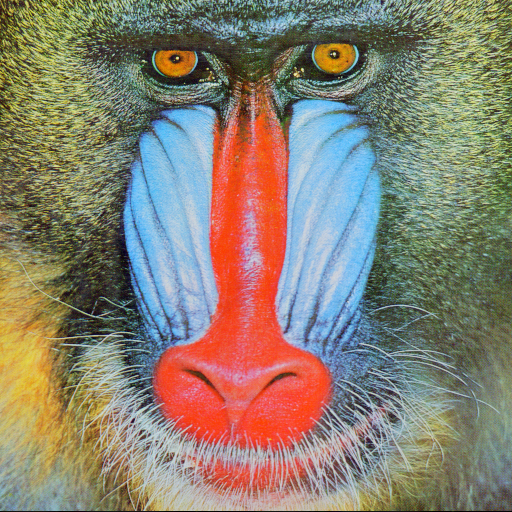
\includegraphics[width=4cm]{../out/cbaboon.png} }}%
	\qquad
	\subfloat[\centering Versão em escala de cinza da imagem Baboon (convertida)]{{ 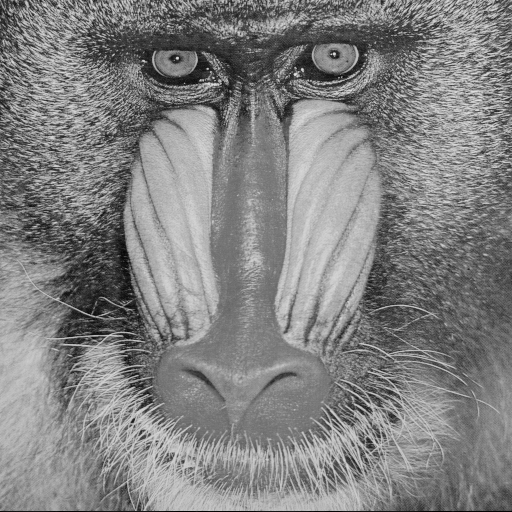
\includegraphics[width=4cm]{../out/baboon.png} }}%	
	\caption{Imagens utilizadas para aplicação das técnicas de meios-tons por difusão de erro.}%	
	\label{fig:imagem:entrada}%
\end{figure}

Para comparação com as imagens resultantes das técinicas de meios-tons por difusão de erro, gerou-se imagens denominadas controle a partir da aplicação da técnica de meio-tom que utiliza apenas o limiar de 128 para tomada de decisão se a um pixel será atribuído o valor zero (0) ou o valor (1). As imagens controle da imagem Baboon nas versões colorida e em escala de cinza são apresentadas na Figura \ref{fig:imagem:controle}.

\begin{figure}[htp]%
	\centering
	
	\subfloat[\centering Imagem controle na versão colorida]{{ 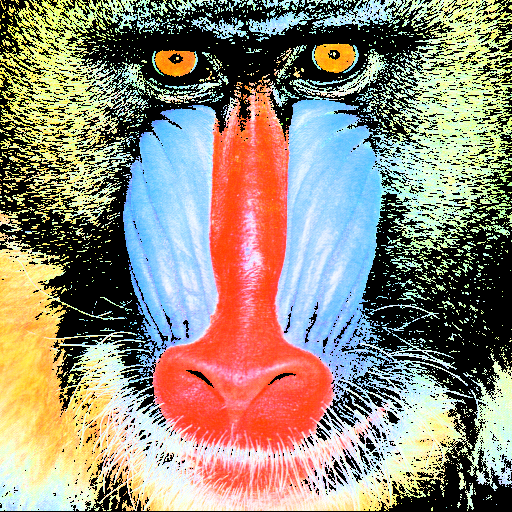
\includegraphics[width=5cm]{../out/cbaboon_control.png} }}%
	\qquad
	\subfloat[\centering Imagem controle na versão em preto e branco]{{ 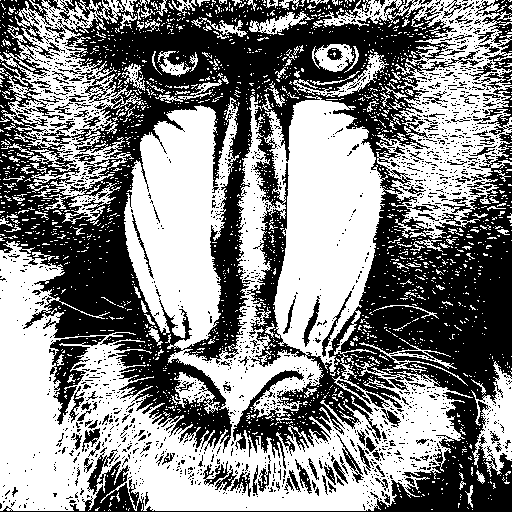
\includegraphics[width=5cm]{../out/baboon_control.png} }}%	
	
	\caption{Imagens controle para comparação com as imagens resultantes da aplicação da técnicas de meios-tons por difusão de erro.}%
	
	\label{fig:imagem:controle}%
\end{figure}

Na sequência, teremos a apresentação das imagens resultantes da aplicação das técnias de meios-tons por difusão de erro sobre a imagem Baboon na sua versão colorida e em escala de cinza.



\subsection{Técnicas de meios-tons sobre images em escala de cinza}
Aqui serão apresentados as imagens resultados da aplicação das técnicas de meios-tons sobre a imagem de entrada em escala de cinza.

\begin{figure}[htp]%
	\centering
    \subfloat[\centering Imagem em meio-tom controle (aplicação apenas do limiar de 128)]{{ 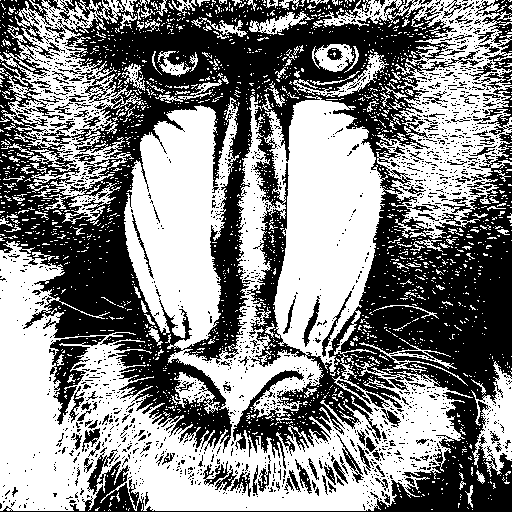
\includegraphics[width=3cm]{../out/baboon_control.png} }}%
	\qquad
	\subfloat[\centering Imagem em meio-tom pela técnica de Floyd e Steinberg]{{ 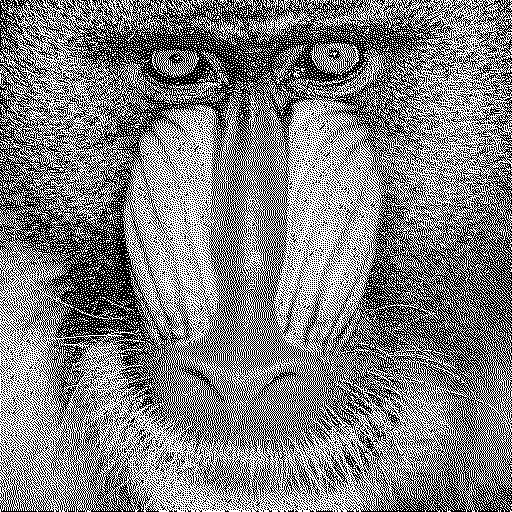
\includegraphics[width=3cm]{../out/baboon_floydsteinberg.png} }}%
	\qquad
    \subfloat[\centering Imagem em meio-tom pela técnica de Stevenson e Arce]{{ 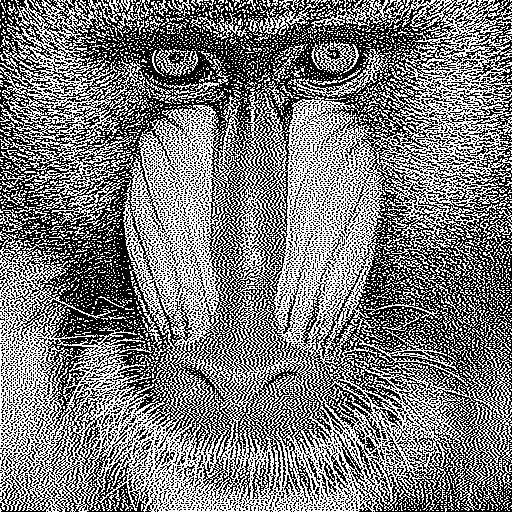
\includegraphics[width=3cm]{../out/baboon_stevensonarce.png} }}%
	
	%\subfloat[\centering ]{{
\includegraphics[width=3cm]{../out/baboonm_plano0_texto1_plano_bits_1_R.png} }}%
	%\qquad
	%\subfloat[\centering ]{{
\includegraphics[width=3cm]{../out/baboonm_plano0_texto1_plano_bits_1_G.png} }}%
	%\qquad
	%\subfloat[\centering ]{{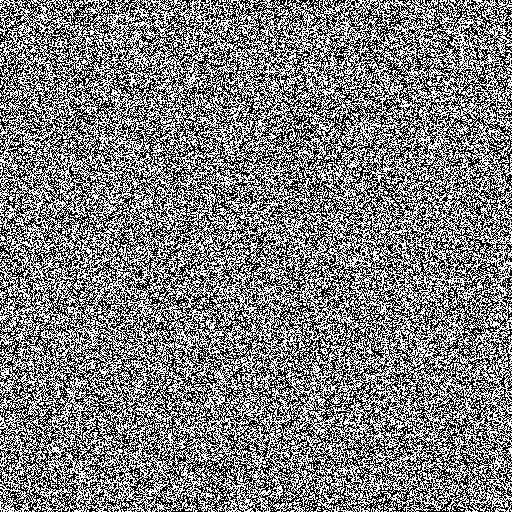
\includegraphics[width=3cm]{../out/baboonm_plano0_texto1_plano_bits_1_B.png} }}%
	%
	%\subfloat[\centering ]{{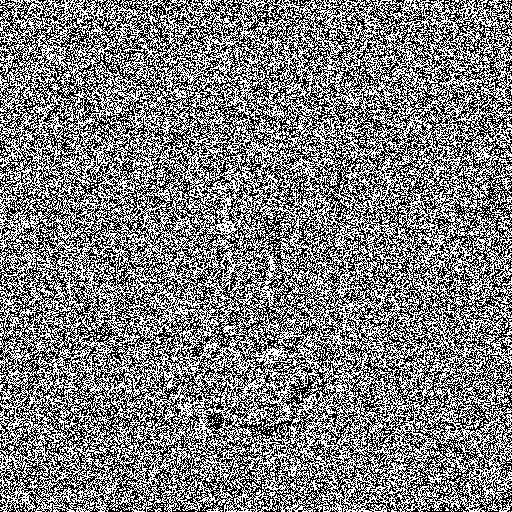
\includegraphics[width=3cm]{../out/baboonm_plano0_texto1_plano_bits_2_R.png} }}%
	%\qquad
	%\subfloat[\centering ]{{
\includegraphics[width=3cm]{../out/baboonm_plano0_texto1_plano_bits_2_G.png} }}%
	%\qquad
	%\subfloat[\centering ]{{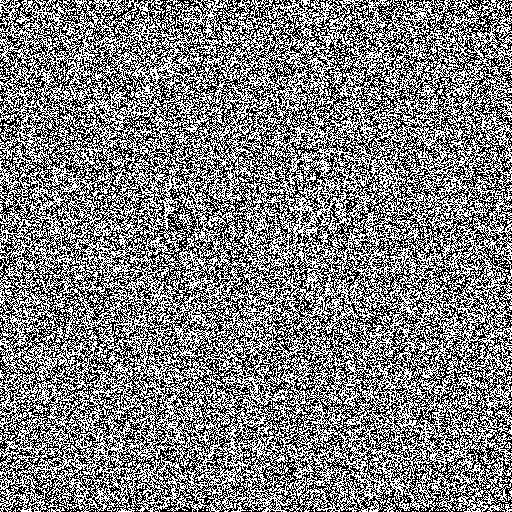
\includegraphics[width=3cm]{../out/baboonm_plano0_texto1_plano_bits_2_B.png} }}%
	%
	%\subfloat[\centering ]{{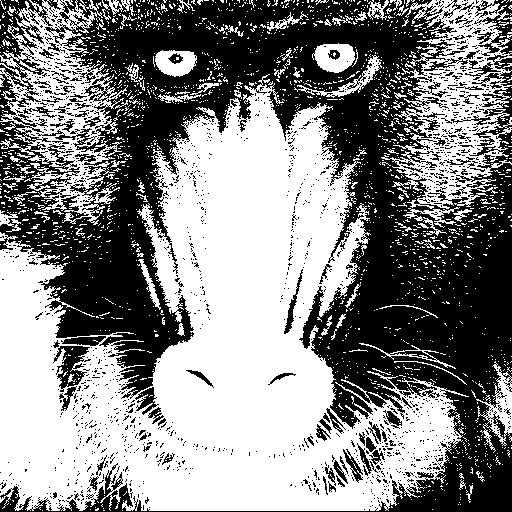
\includegraphics[width=3cm]{../out/baboonm_plano0_texto1_plano_bits_7_R.png} }}%
	%\qquad
	%\subfloat[\centering ]{{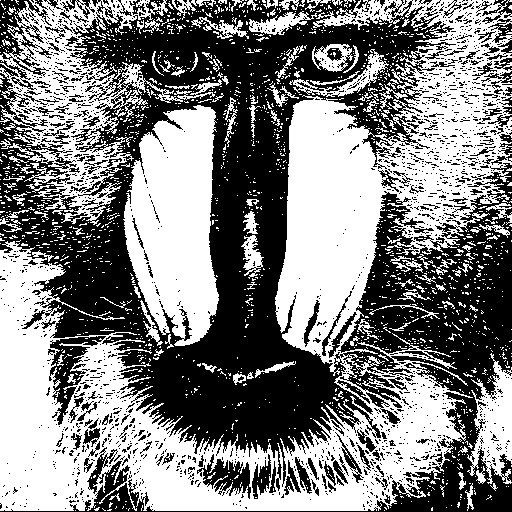
\includegraphics[width=3cm]{../out/baboonm_plano0_texto1_plano_bits_7_G.png} }}%
	%\qquad
	%\subfloat[\centering Plano de bits 7 do canal B da Baboon com mensagem escondida]{{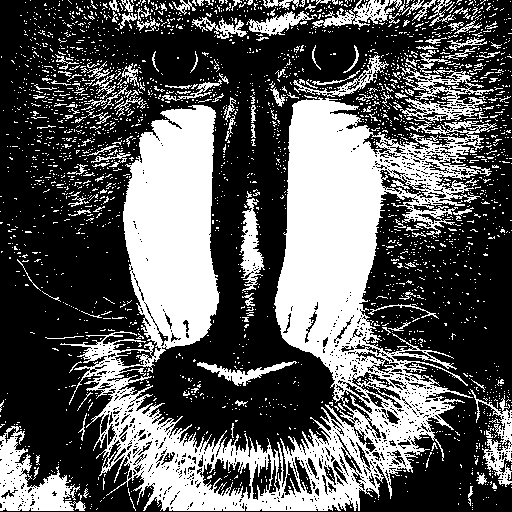
\includegraphics[width=3cm]{../out/baboonm_plano0_texto1_plano_bits_7_B.png} }}%

	\caption{Planos de bits da imagem do Baboon modificada pelos bits da mensagem do arquivo \textbf{texto1.txt}.}%
	\label{fig:imagem:plano:baboon}%
\end{figure}	



	
%\begin{figure}[htp]%
%\centering
%\subfloat[\centering Baboon com mensagem escondida (out/baboonm\_plano0\_texto1.png)]{{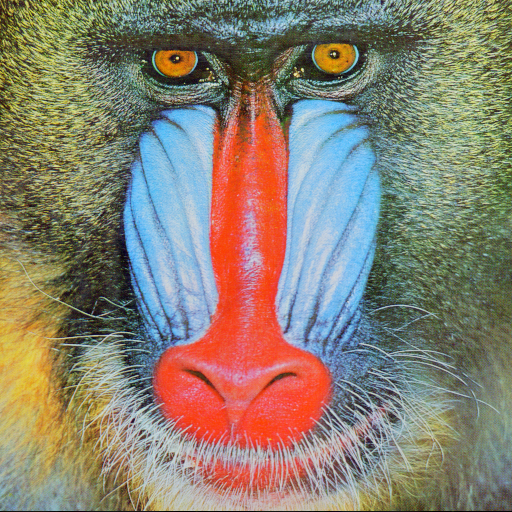
\includegraphics[width=5cm]{../out/baboonm_plano0_texto1.png} }}%
%\qquad
%\subfloat[\centering Watch com mensagem escondida (out/watchm\_plano0\_texto1.png)]{{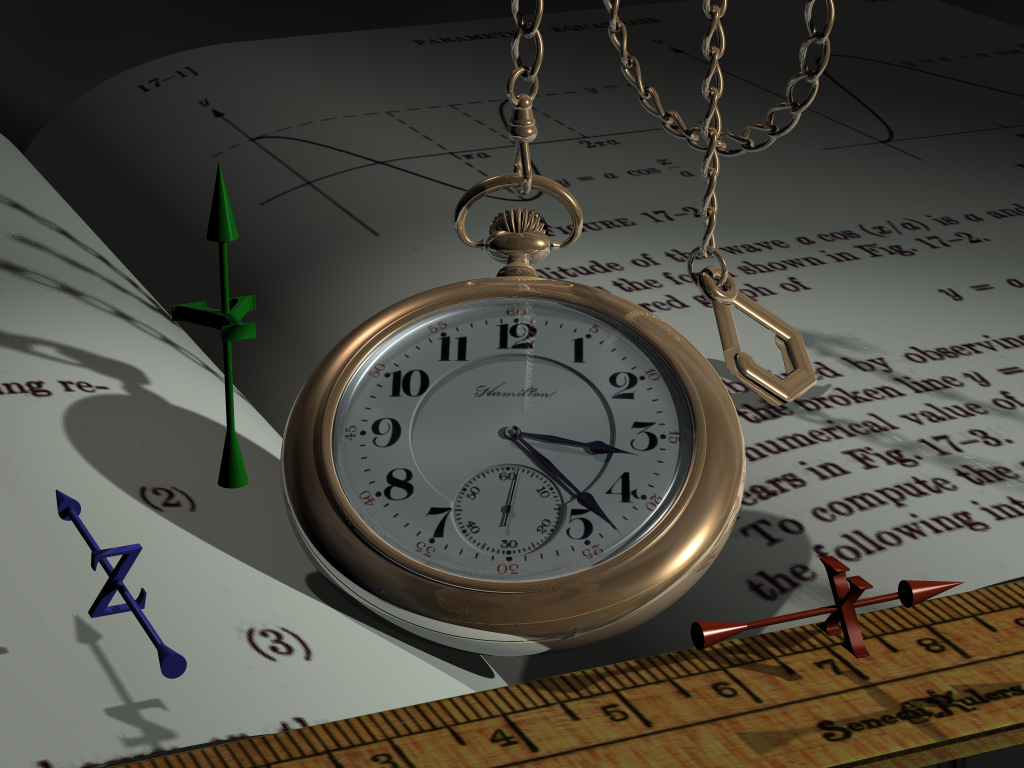
\includegraphics[width=5cm]{../out/watchm_plano0_texto1.png} }}%
%\caption{Imagens que apresentam mensagem escondida do arquivo \textbf{texto1.txt}.}%
%\label{fig:imagem:saida}%
%\end{figure}	
%
%\newpage\noindent
%Os comandos utilizados para ocultação de mensagem contida no arquivo \textbf{texto\_longo\_1.txt} foram:
%
%\lstinline{python3 codificar.py -imagem_entrada=png/baboon.png -texto_entrada=txt/texto_longo_1.txt -planos_bits=0};
%
%\lstinline{python3 codificar.py -imagem_entrada=png/watch.png -texto_entrada=txt/texto_longo_1.txt -planos_bits=0}.
%
%\noindent
%As imagens resultantes com a mensagem escondida estão apresentadas na Figura \ref{fig:imagem:saida2}.
%
%\begin{figure}[htp]%
%	\centering
%	\subfloat[\centering Baboon com mensagem escondida (/out/baboonm\_plano0\_texto\_longo\_1.png)]{{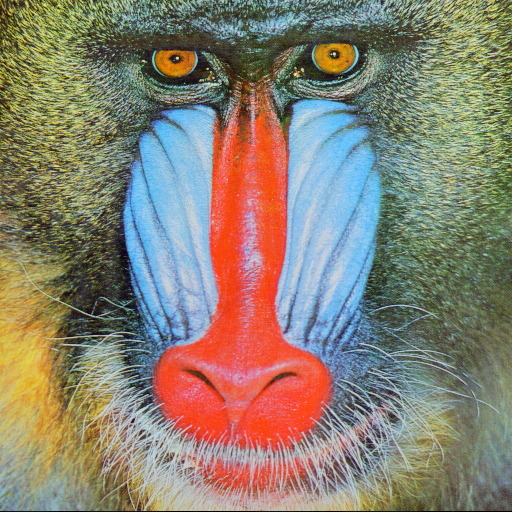
\includegraphics[width=5cm]{../out/baboonm_plano0_texto_longo_1.png} }}%
%	\qquad
%	\subfloat[\centering Watch com mensagem escondida (out/watchm\_plano0\_texto\_longo\_1.png)]{{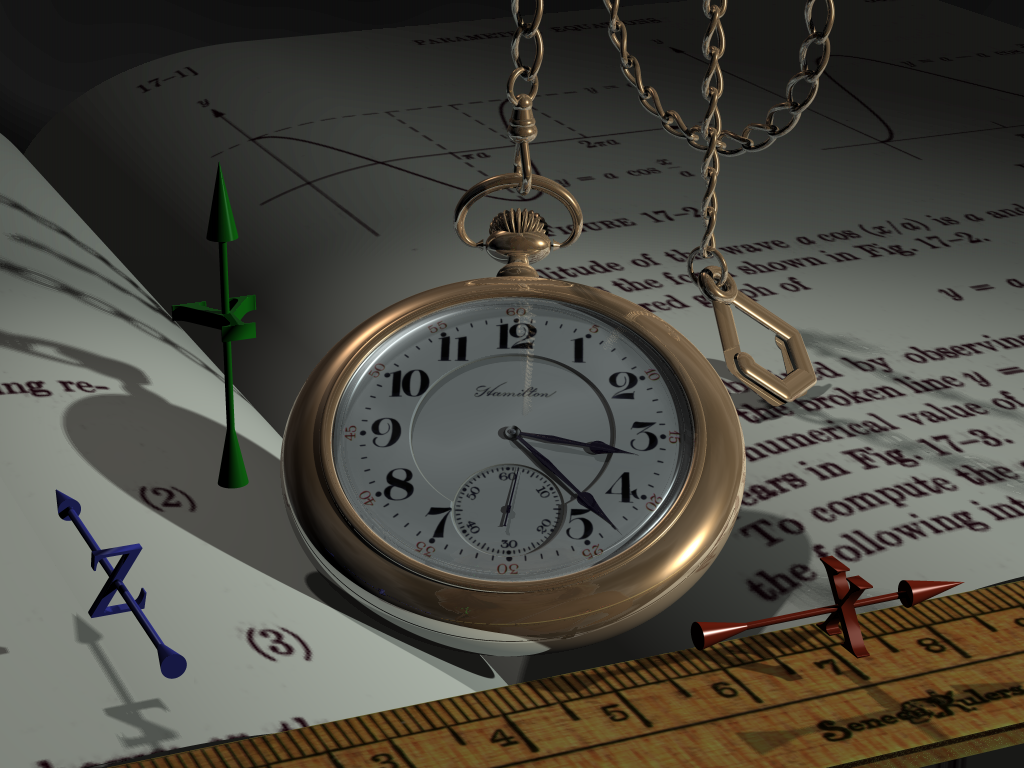
\includegraphics[width=5cm]{../out/watchm_plano0_texto_longo_1.png} }}%
%	\caption{Imagens que apresentam mensagem escondida do arquivo do \textbf{texto\_longo\_1.txt}.}%
%	\label{fig:imagem:saida2}%
%\end{figure}
%
%
%Nota-se que visualmente, essas imagens, apesar de modificadas pelos bits da mensagem escondida, não apresentam alterações visuais perceptíveis ao olho humano. Vamos visualizar os planos 0, 1, 2 e 7 dessas imagens para cada umas das duas mensagens \textbf{texto1.txt} e \textbf{texto\_longo\_1.txt}. 
%
%
%\subsection{Planos de bits da imagem Baboon e Watch modifica pela mensagem contida no arquivo texto1.txt}
%
%Começaremos visualizando os planos de bits da imagem do Baboon modificada. Os planos apresentados serão os 0, 1, 2, e 7 (0 menos significativo, 7 o mais significativo). As imagens dos planos de bits podem ser visualizadas na Figura \ref{fig:imagem:plano:baboon}.
%
%\begin{figure}[htp]%
%	\centering
%	\subfloat[\centering Plano de bits 0 do canal R da Baboon com mensagem escondida]{{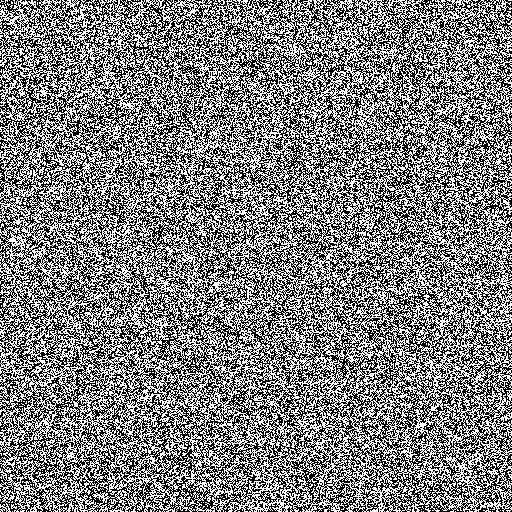
\includegraphics[width=3cm]{../out/baboonm_plano0_texto1_plano_bits_0_R.png} }}%
%	\qquad
%	\subfloat[\centering Plano de bits 0 do canal G da Baboon com mensagem escondida]{{
\includegraphics[width=3cm]{../out/baboonm_plano0_texto1_plano_bits_0_G.png} }}%
%	\qquad
%	\subfloat[\centering Plano de bits 0 do canal B da Baboon com mensagem escondida]{{
\includegraphics[width=3cm]{../out/baboonm_plano0_texto1_plano_bits_0_B.png} }}%
%	
%	\subfloat[\centering Plano de bits 1 do canal R da Baboon com mensagem escondida]{{
\includegraphics[width=3cm]{../out/baboonm_plano0_texto1_plano_bits_1_R.png} }}%
%	\qquad
%	\subfloat[\centering Plano de bits 1 do canal G da Baboon com mensagem escondida]{{
\includegraphics[width=3cm]{../out/baboonm_plano0_texto1_plano_bits_1_G.png} }}%
%	\qquad
%	\subfloat[\centering Plano de bits 1 do canal B da Baboon com mensagem escondida]{{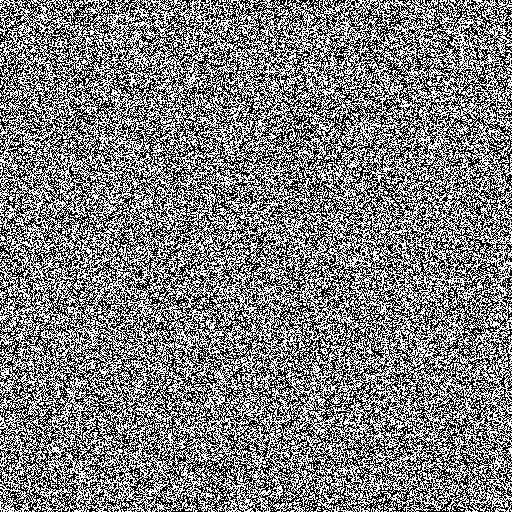
\includegraphics[width=3cm]{../out/baboonm_plano0_texto1_plano_bits_1_B.png} }}%
%	
%	\subfloat[\centering Plano de bits 2 do canal R da Baboon com mensagem escondida]{{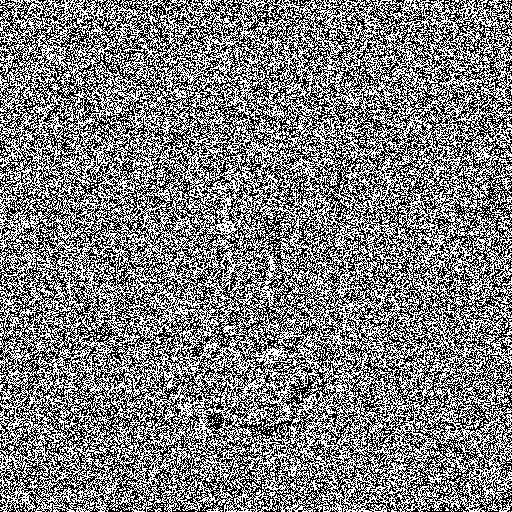
\includegraphics[width=3cm]{../out/baboonm_plano0_texto1_plano_bits_2_R.png} }}%
%	\qquad
%	\subfloat[\centering Plano de bits 2 do canal G da Baboon com mensagem escondida]{{
\includegraphics[width=3cm]{../out/baboonm_plano0_texto1_plano_bits_2_G.png} }}%
%	\qquad
%	\subfloat[\centering Plano de bits 2 do canal B da Baboon com mensagem escondida]{{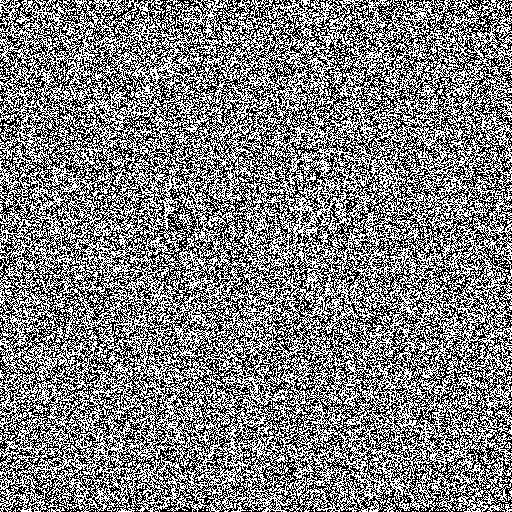
\includegraphics[width=3cm]{../out/baboonm_plano0_texto1_plano_bits_2_B.png} }}%
%	
%	\subfloat[\centering Plano de bits 7 do canal R da Baboon com mensagem escondida]{{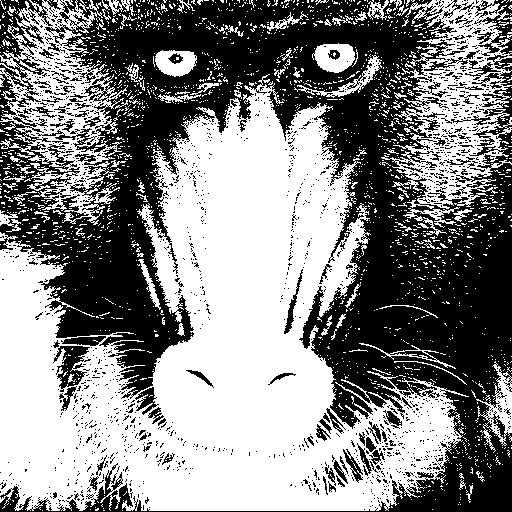
\includegraphics[width=3cm]{../out/baboonm_plano0_texto1_plano_bits_7_R.png} }}%
%	\qquad
%	\subfloat[\centering Plano de bits 7 do canal G da Baboon com mensagem escondida]{{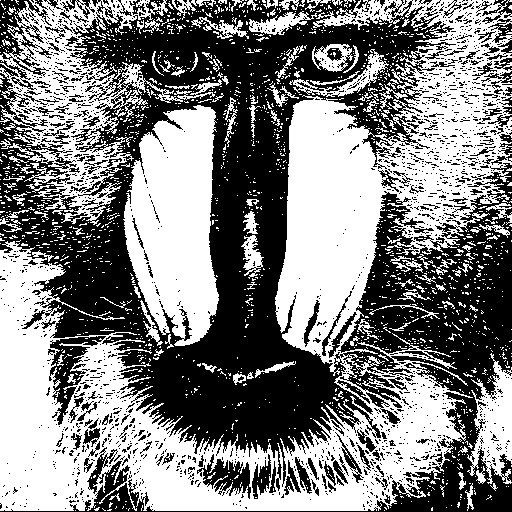
\includegraphics[width=3cm]{../out/baboonm_plano0_texto1_plano_bits_7_G.png} }}%
%	\qquad
%	\subfloat[\centering Plano de bits 7 do canal B da Baboon com mensagem escondida]{{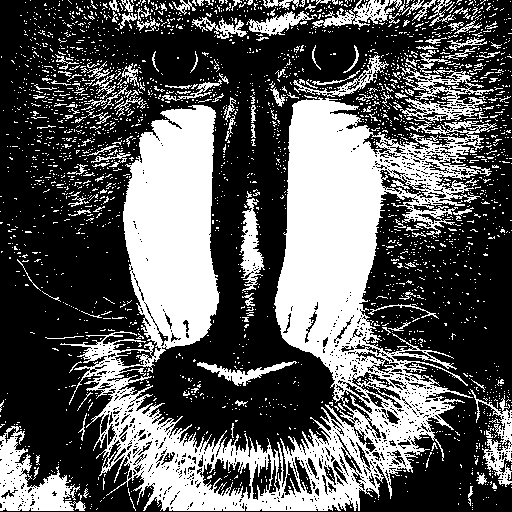
\includegraphics[width=3cm]{../out/baboonm_plano0_texto1_plano_bits_7_B.png} }}%
%
%	\caption{Planos de bits da imagem do Baboon modificada pelos bits da mensagem do arquivo \textbf{texto1.txt}.}%
%	\label{fig:imagem:plano:baboon}%
%\end{figure}	
%
%
%Para as imagens apresentadas na Figura \ref{fig:imagem:plano:baboon}, notamos que não é possível visualmente verificar que a imagem foi modificada a partir da análise visual dos seus planos de bits. Essa condição deve ser propiciada tanto pela ruído apresentado nos planos de bits menos significativos quanto pelo tamanho da mensagem que é pequeno. Também podemos perceber que os planos bits menos significativos carregam menos informações da composição da imagem do que os planos de bits mais significativos. Logo, é por isso que modificar esse bits (os menos significativos) não altera perceptivelmente a imagem de saída.
%
%\newpage
%Agora vamos verificar o planos de bits 0, 1, 2 e 7 da imagem Watch modificada. Esses planos de bits estão apresentados na Figura \ref{fig:imagem:plano:watch}. 
%
%\begin{figure}[htp]%
%	\centering
%	\subfloat[\centering Plano de bits 0 do canal R da Watch com mensagem escondida]{{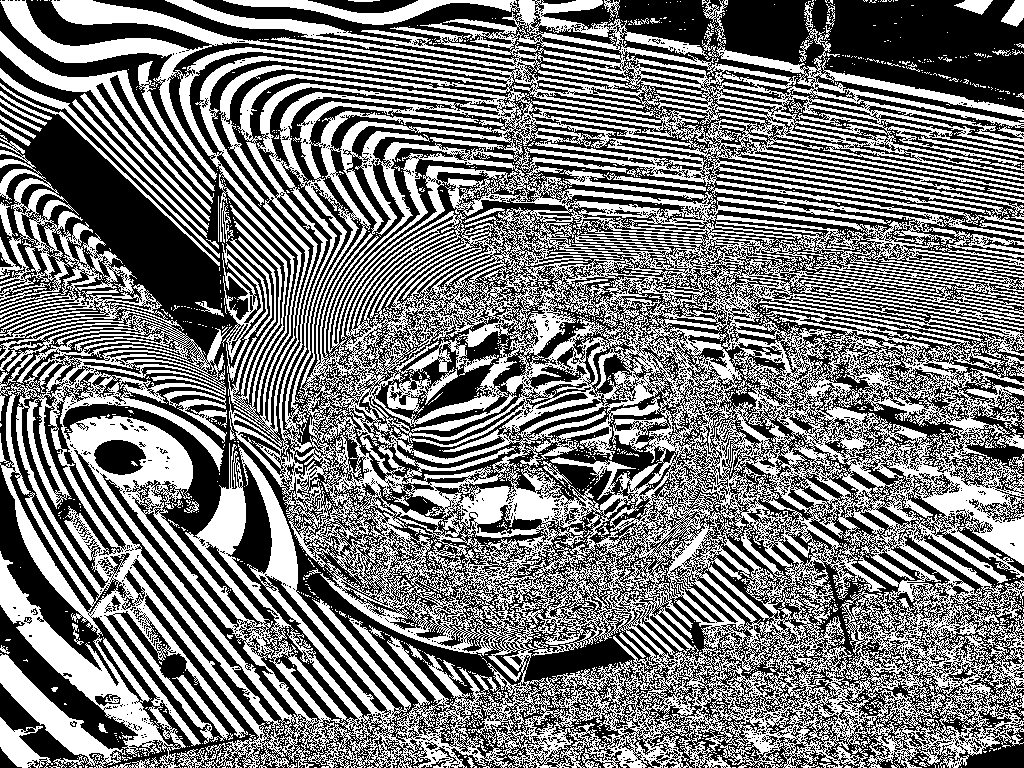
\includegraphics[width=3cm]{../out/watchm_plano0_texto1_plano_bits_0_R.png} }}%
%	\qquad
%	\subfloat[\centering Plano de bits 0 do canal G da Watch com mensagem escondida]{{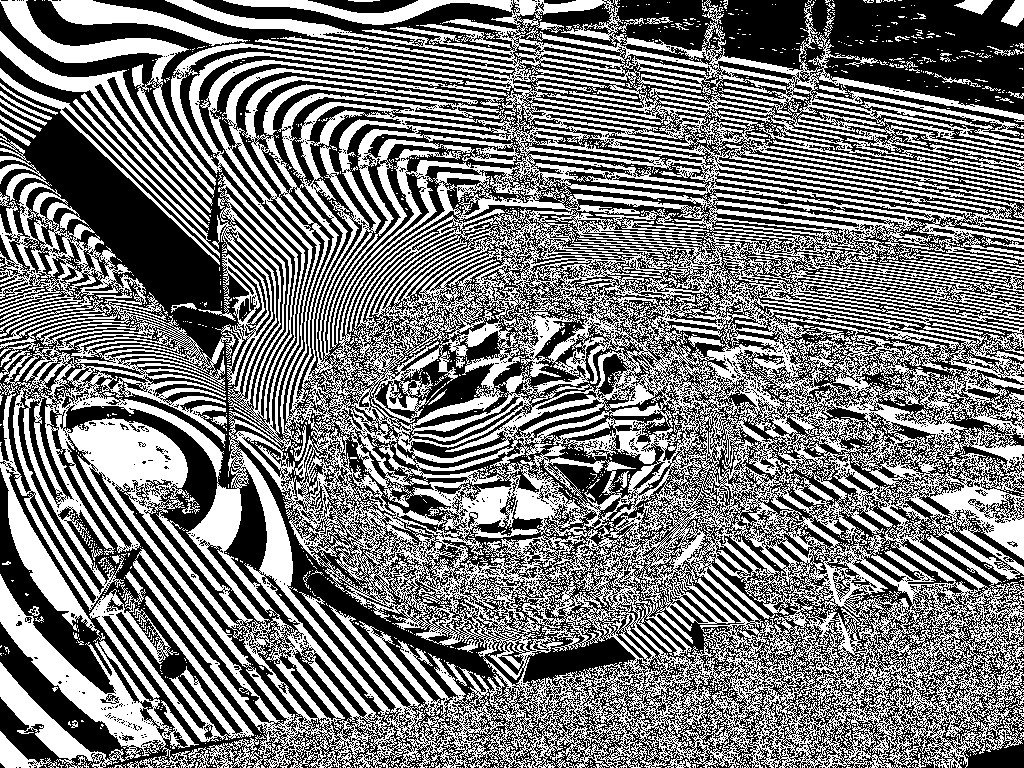
\includegraphics[width=3cm]{../out/watchm_plano0_texto1_plano_bits_0_G.png} }}%
%	\qquad
%	\subfloat[\centering Plano de bits 0 do canal B da Watch com mensagem escondida]{{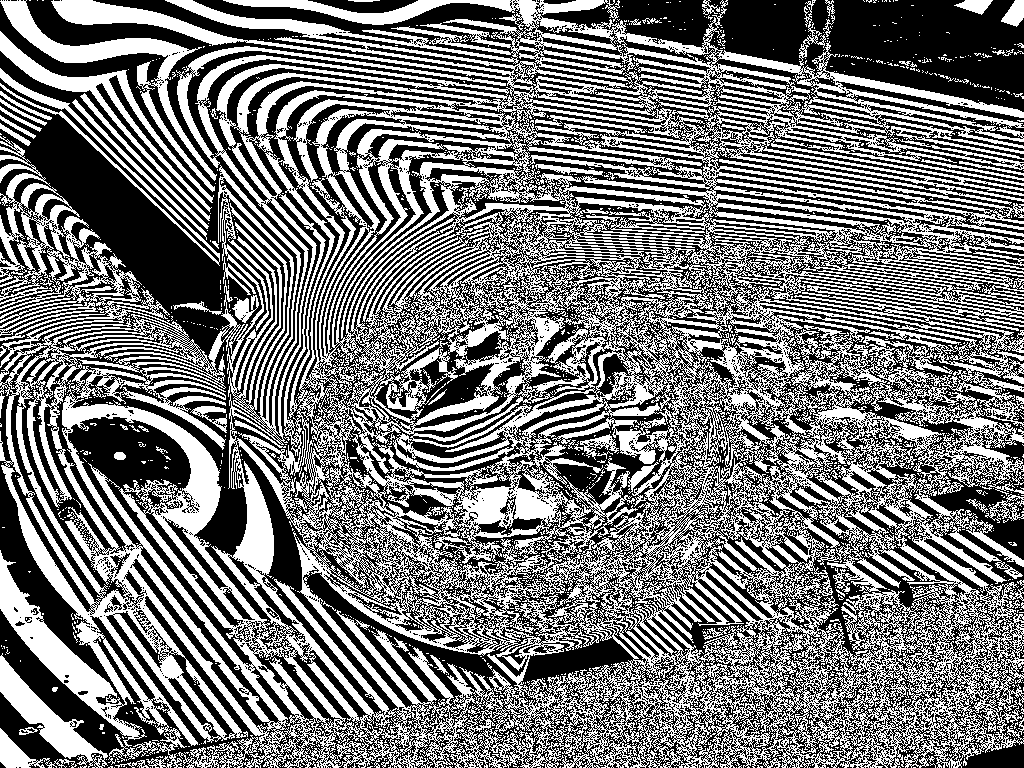
\includegraphics[width=3cm]{../out/watchm_plano0_texto1_plano_bits_0_B.png} }}%
%	
%	\subfloat[\centering Plano de bits 1 do canal R da Watch com mensagem escondida]{{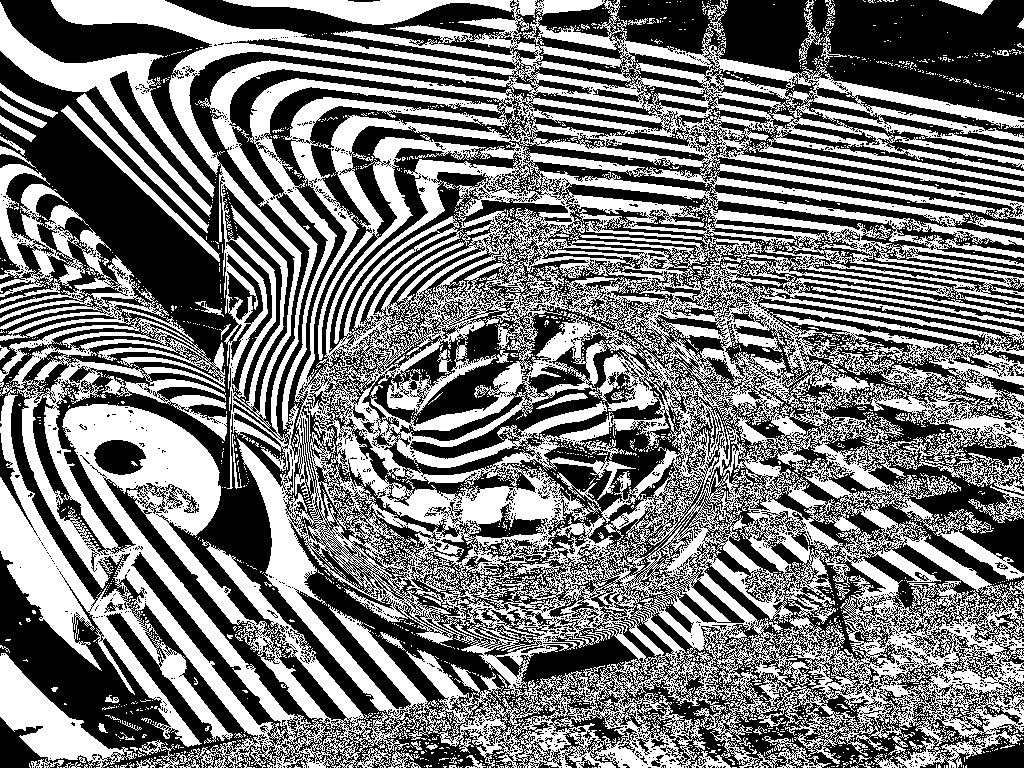
\includegraphics[width=3cm]{../out/watchm_plano0_texto1_plano_bits_1_R.png} }}%
%	\qquad
%	\subfloat[\centering Plano de bits 1 do canal G da Watch com mensagem escondida]{{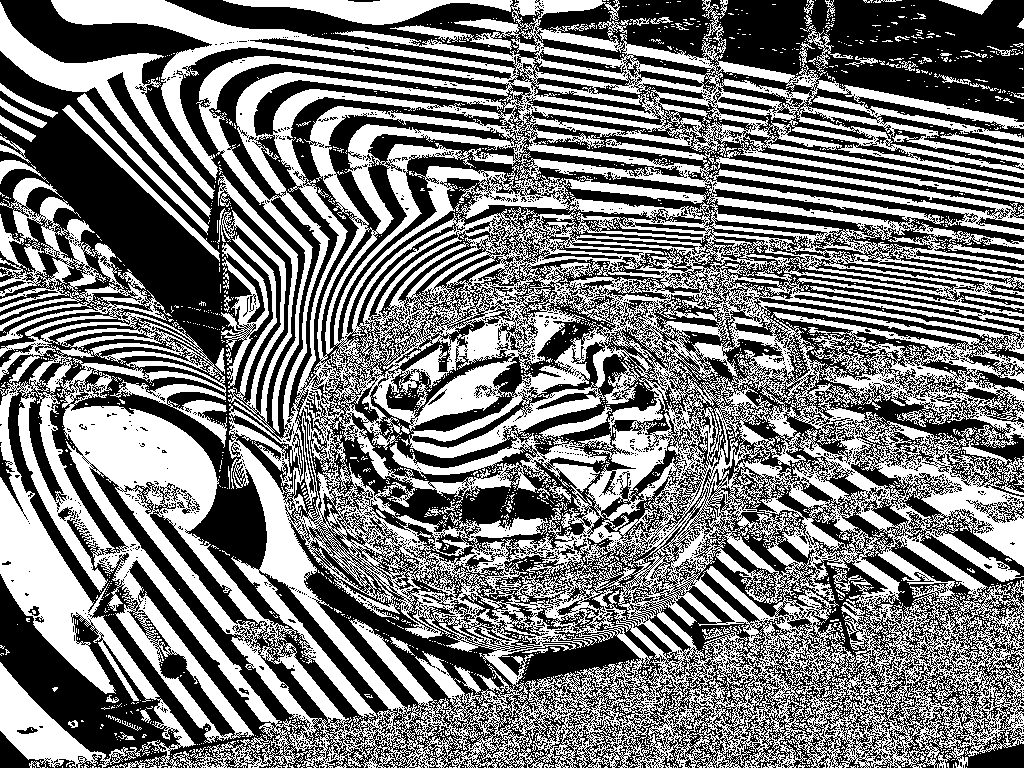
\includegraphics[width=3cm]{../out/watchm_plano0_texto1_plano_bits_1_G.png} }}%
%	\qquad
%	\subfloat[\centering Plano de bits 1 do canal B da Watch com mensagem escondida]{{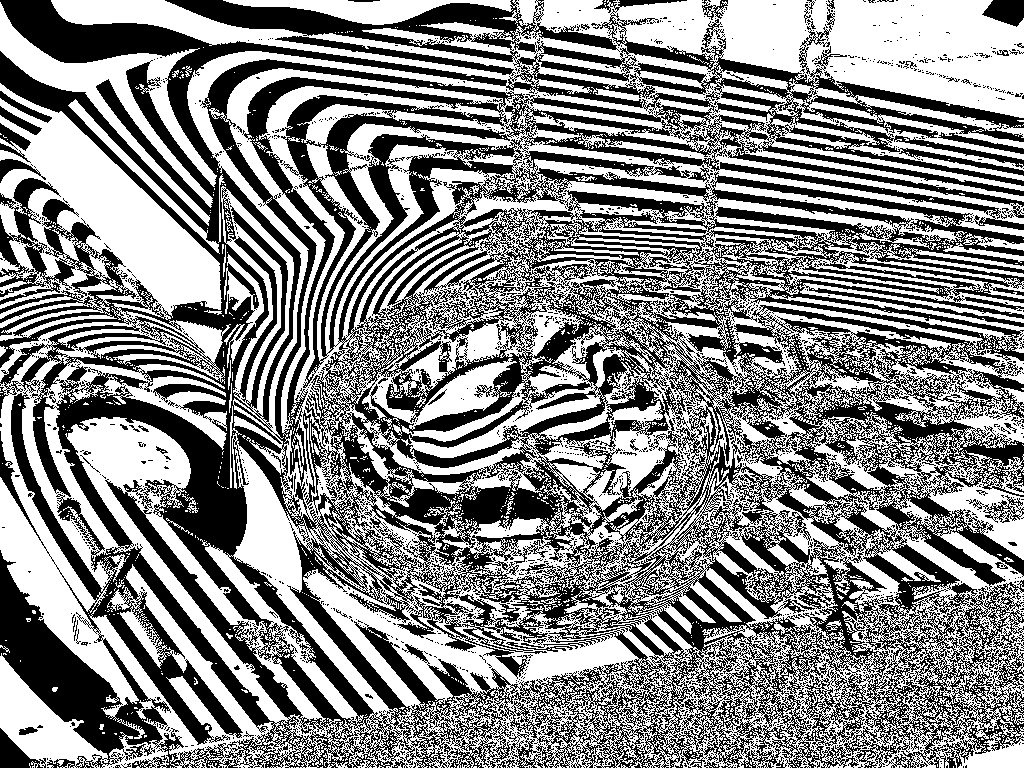
\includegraphics[width=3cm]{../out/watchm_plano0_texto1_plano_bits_1_B.png} }}%
%	
%	\subfloat[\centering Plano de bits 2 do canal R da Watch com mensagem escondida]{{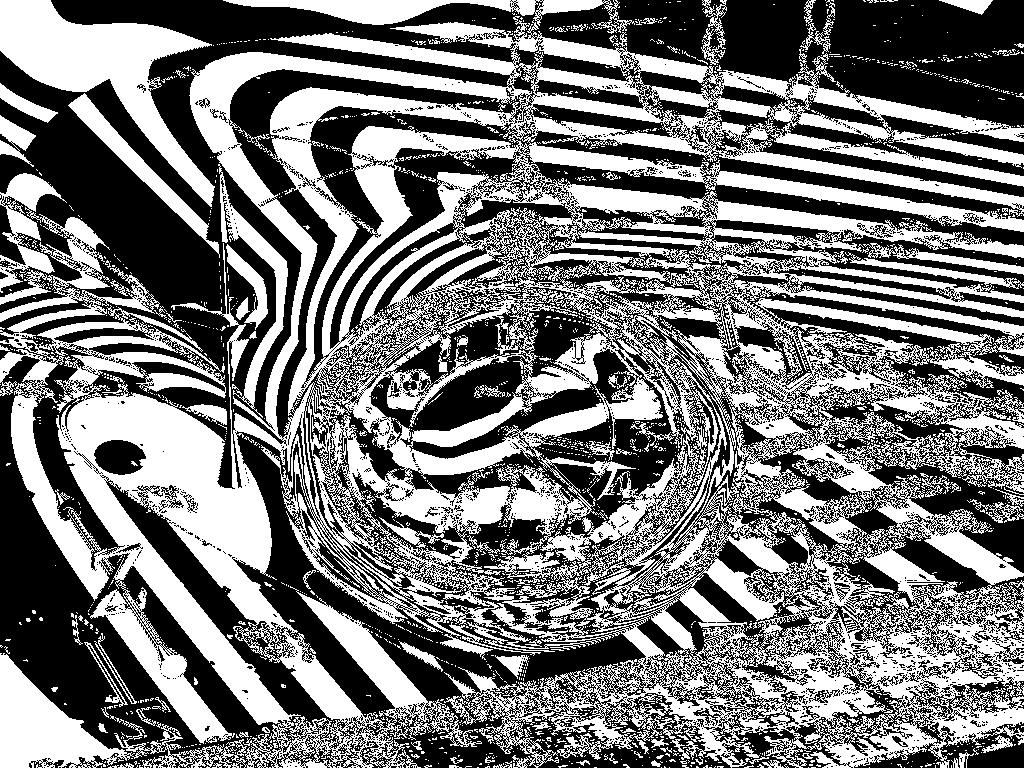
\includegraphics[width=3cm]{../out/watchm_plano0_texto1_plano_bits_2_R.png} }}%
%	\qquad
%	\subfloat[\centering Plano de bits 2 do canal G da Watch com mensagem escondida]{{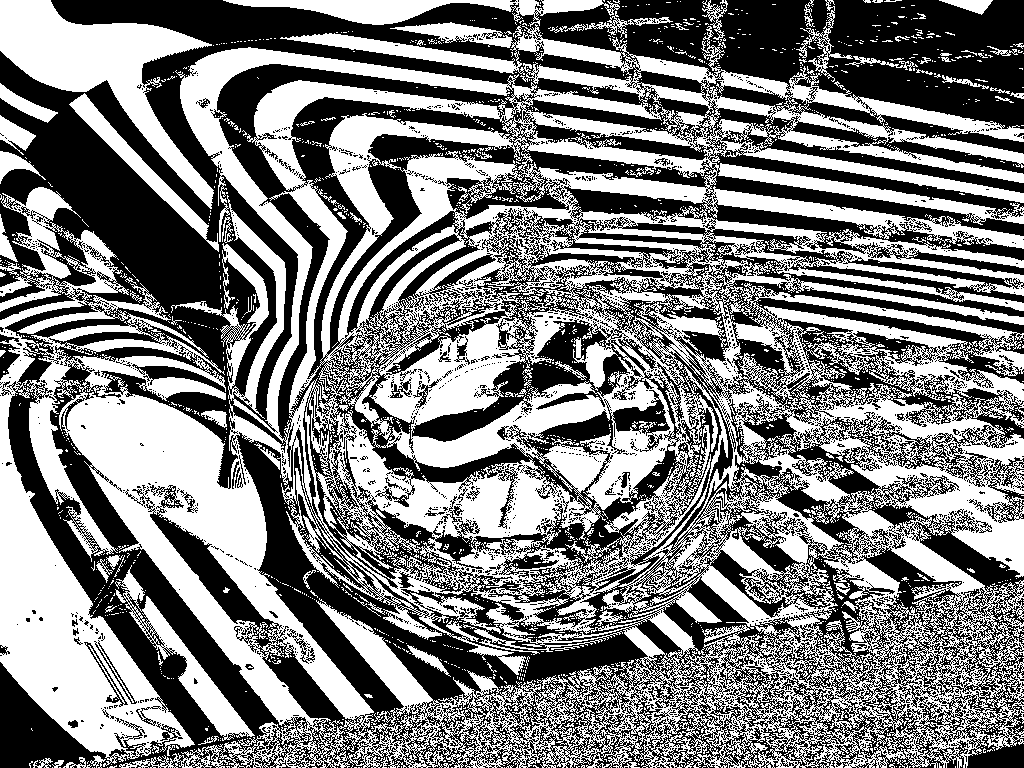
\includegraphics[width=3cm]{../out/watchm_plano0_texto1_plano_bits_2_G.png} }}%
%	\qquad
%	\subfloat[\centering Plano de bits 2 do canal B da Watch com mensagem escondida]{{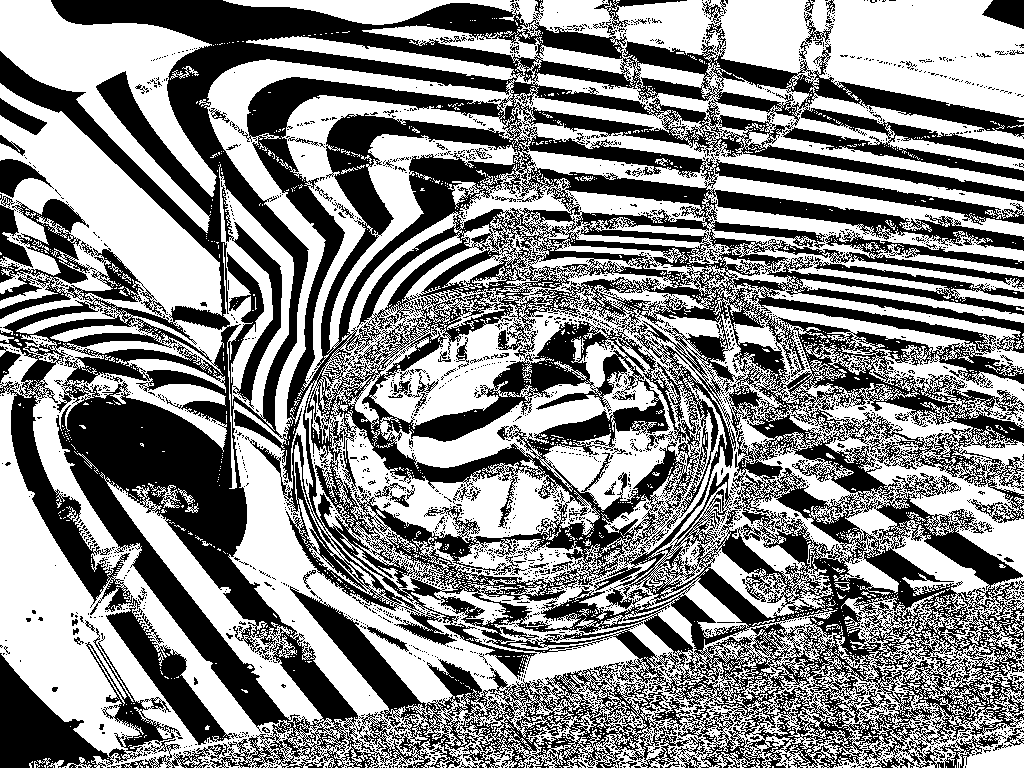
\includegraphics[width=3cm]{../out/watchm_plano0_texto1_plano_bits_2_B.png} }}%
%	
%	\subfloat[\centering Plano de bits 7 do canal R da Watch com mensagem escondida]{{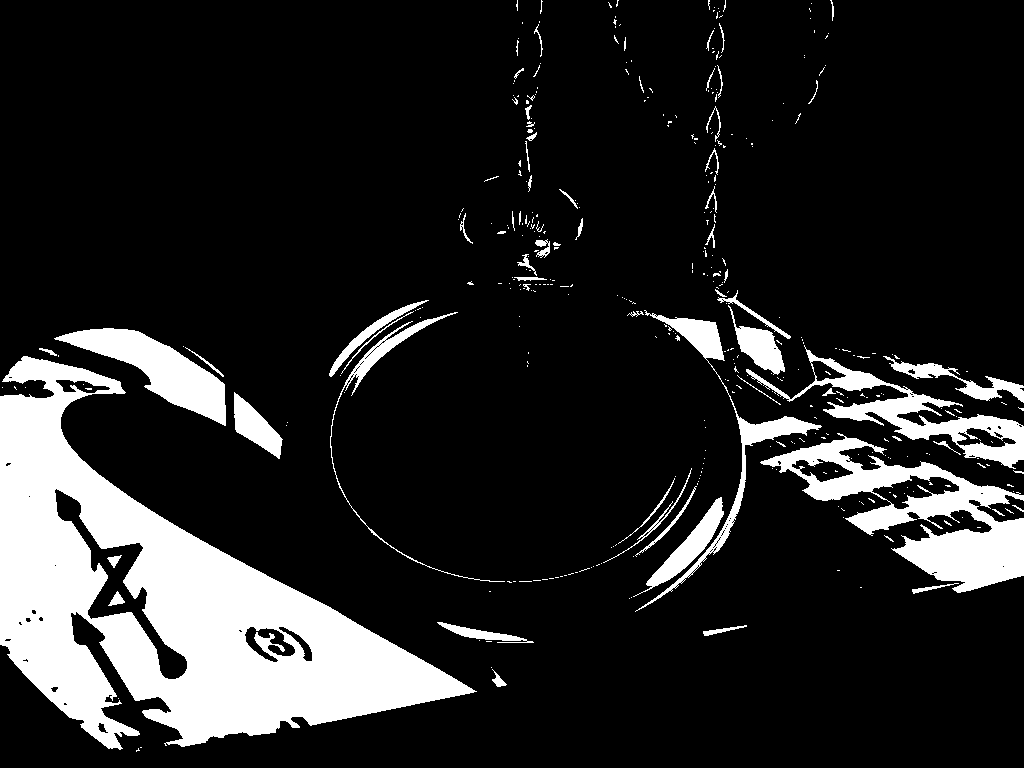
\includegraphics[width=3cm]{../out/watchm_plano0_texto1_plano_bits_7_R.png} }}%
%	\qquad
%	\subfloat[\centering Plano de bits 7 do canal G da Watch com mensagem escondida]{{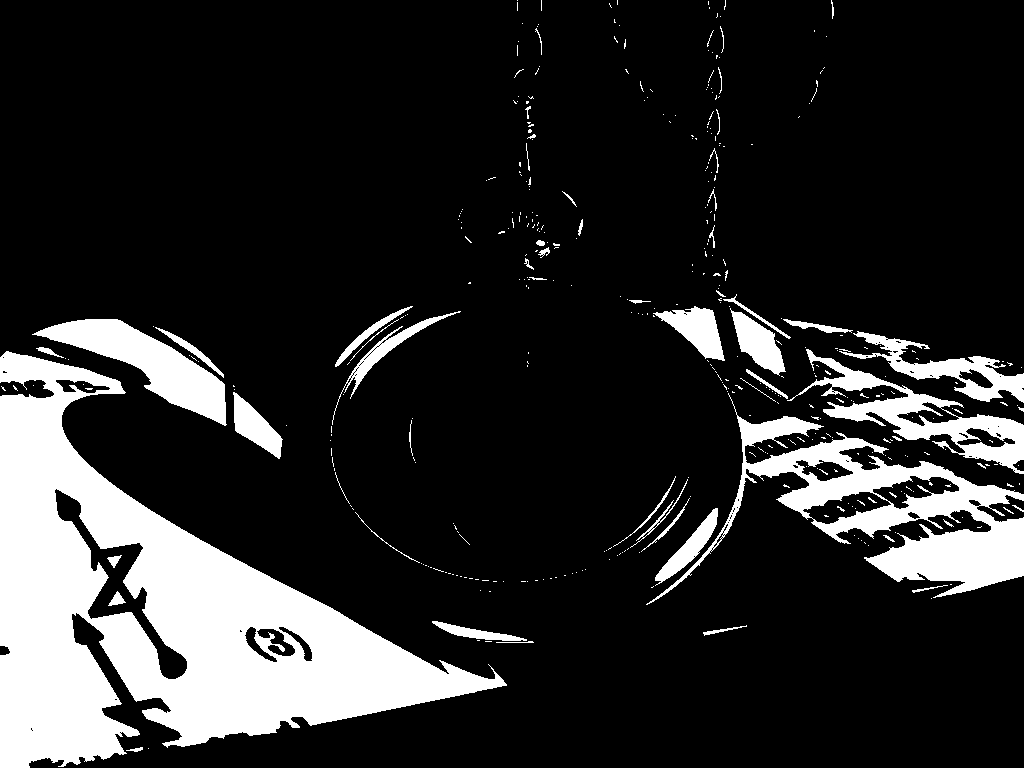
\includegraphics[width=3cm]{../out/watchm_plano0_texto1_plano_bits_7_G.png} }}%
%	\qquad
%	\subfloat[\centering Plano de bits 7 do canal B da Watch com mensagem escondida]{{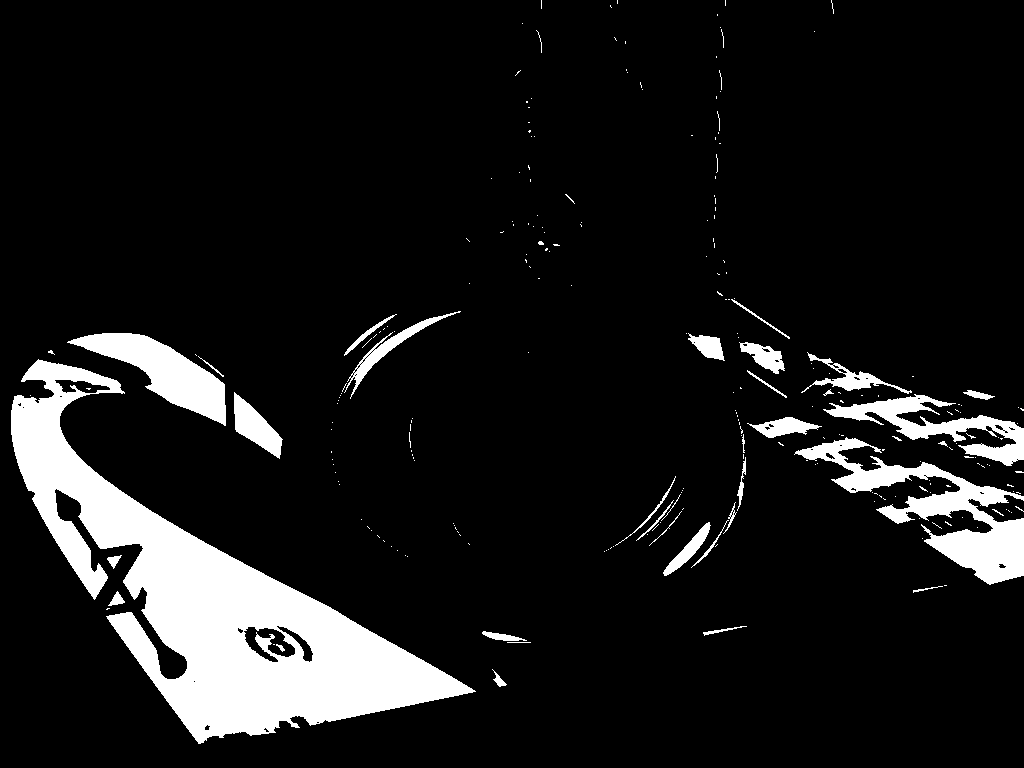
\includegraphics[width=3cm]{../out/watchm_plano0_texto1_plano_bits_7_B.png} }}%
%	
%	\caption{Planos de bits da imagem do Watch modificada pelos bits da mensagem do arquivo \textbf{texto1.txt}.}%
%	\label{fig:imagem:plano:watch}%
%\end{figure}
%
%No caso dessa imagem, é possível notar uma alteração dos padrões de bits apresentados no seu plano de bits 0 (que é o plano onde a mensagem foi inserida). A visualização dessa quebra de padrão está dificuldade pelo tamanho da imagem, mas um olhar atento ainda é capaz de verificá-lo (olhar canto superior esquerdo da primeira linha de imagens).
%
%\subsection{Planos de bits da imagem Baboon e Watch modifica pela mensagem contida no arquivo texto\_longo\_1.txt}
%
%Começaremos visualizando os planos de bits da imagem do Baboon modificada. Os planos apresentados serão o 0, 1, 2, e 7 (0 menos significativo, 7 o mais significativo). As imagens dos planos de bits podem ser visualizadas na Figura \ref{fig:imagem:plano:baboon2}.
%
%\begin{figure}[htp]%
%	\centering
%	\subfloat[\centering Plano de bits 0 do canal R da Baboon com mensagem escondida]{{
\includegraphics[width=3cm]{../out/baboonm_plano0_texto_longo_1_plano_bits_0_R.png} }}%
%	\qquad
%	\subfloat[\centering Plano de bits 0 do canal G da Baboon com mensagem escondida]{{
\includegraphics[width=3cm]{../out/baboonm_plano0_texto_longo_1_plano_bits_0_G.png} }}%
%	\qquad
%	\subfloat[\centering Plano de bits 0 do canal B da Baboon com mensagem escondida]{{
\includegraphics[width=3cm]{../out/baboonm_plano0_texto_longo_1_plano_bits_0_B.png} }}%
%	
%	\subfloat[\centering Plano de bits 1 do canal R da Baboon com mensagem escondida]{{
\includegraphics[width=3cm]{../out/baboonm_plano0_texto_longo_1_plano_bits_1_R.png} }}%
%	\qquad
%	\subfloat[\centering Plano de bits 1 do canal G da Baboon com mensagem escondida]{{
\includegraphics[width=3cm]{../out/baboonm_plano0_texto_longo_1_plano_bits_1_G.png} }}%
%	\qquad
%	\subfloat[\centering Plano de bits 1 do canal B da Baboon com mensagem escondida]{{\includegraphics[width=3cm]{../out/baboonm_plano0_texto_longo_1_plano_bits_1_B.png} }}%
%	
%	\subfloat[\centering Plano de bits 2 do canal R da Baboon com mensagem escondida]{{\includegraphics[width=3cm]{../out/baboonm_plano0_texto_longo_1_plano_bits_2_R.png} }}%
%	\qquad
%	\subfloat[\centering Plano de bits 2 do canal G da Baboon com mensagem escondida]{{\includegraphics[width=3cm]{../out/baboonm_plano0_texto_longo_1_plano_bits_2_G.png} }}%
%	\qquad
%	\subfloat[\centering Plano de bits 2 do canal B da Baboon com mensagem escondida]{{\includegraphics[width=3cm]{../out/baboonm_plano0_texto_longo_1_plano_bits_2_B.png} }}%
%	
%	\subfloat[\centering Plano de bits 7 do canal R da Baboon com mensagem escondida]{{\includegraphics[width=3cm]{../out/baboonm_plano0_texto_longo_1_plano_bits_7_R.png} }}%
%	\qquad
%	\subfloat[\centering Plano de bits 7 do canal G da Baboon com mensagem escondida]{{\includegraphics[width=3cm]{../out/baboonm_plano0_texto_longo_1_plano_bits_7_G.png} }}%
%	\qquad
%	\subfloat[\centering Plano de bits 7 do canal B da Baboon com mensagem escondida]{{\includegraphics[width=3cm]{../out/baboonm_plano0_texto_longo_1_plano_bits_7_B.png} }}%
%	
%	\caption{Planos de bits da imagem do Baboon modificada pelos bits da mensagem do arquivo \textbf{texto\_longo\_1.txt}.}%
%	\label{fig:imagem:plano:baboon2}%
%\end{figure}
%
%Para as imagens apresentadas na Figura \ref{fig:imagem:plano:baboon2}, notamos que é possível visualmente verificar que a imagem foi modificada a partir da análise visual dos seus planos de bits. Logo, para mensagens muito grandes, pode-se constatar que é possível verificar que uma imagem foi modificada pela análise dos padrões dos seus planos de bits.
%
%\newpage
%Agora vamos verificar o planos de bits 0, 1, 2 e 7 da imagem Watch modificada. Esses planos de bits estão apresentados na Figura \ref{fig:imagem:plano:watch2}. 
%
%\begin{figure}[htp]%
%	\centering
%	\subfloat[\centering Plano de bits 0 do canal R da Watch com mensagem escondida]{{\includegraphics[width=3cm]{../out/watchm_plano0_texto_longo_1_plano_bits_0_R.png} }}%
%	\qquad
%	\subfloat[\centering Plano de bits 0 do canal G da Watch com mensagem escondida]{{\includegraphics[width=3cm]{../out/watchm_plano0_texto_longo_1_plano_bits_0_G.png} }}%
%	\qquad
%	\subfloat[\centering Plano de bits 0 do canal B da Watch com mensagem escondida]{{\includegraphics[width=3cm]{../out/watchm_plano0_texto_longo_1_plano_bits_0_B.png} }}%
%	
%	\subfloat[\centering Plano de bits 1 do canal R da Watch com mensagem escondida]{{\includegraphics[width=3cm]{../out/watchm_plano0_texto_longo_1_plano_bits_1_R.png} }}%
%	\qquad
%	\subfloat[\centering Plano de bits 1 do canal G da Watch com mensagem escondida]{{\includegraphics[width=3cm]{../out/watchm_plano0_texto_longo_1_plano_bits_1_G.png} }}%
%	\qquad
%	\subfloat[\centering Plano de bits 1 do canal B da Watch com mensagem escondida]{{\includegraphics[width=3cm]{../out/watchm_plano0_texto_longo_1_plano_bits_1_B.png} }}%
%	
%	\subfloat[\centering Plano de bits 2 do canal R da Watch com mensagem escondida]{{\includegraphics[width=3cm]{../out/watchm_plano0_texto_longo_1_plano_bits_2_R.png} }}%
%	\qquad
%	\subfloat[\centering Plano de bits 2 do canal G da Watch com mensagem escondida]{{\includegraphics[width=3cm]{../out/watchm_plano0_texto_longo_1_plano_bits_2_G.png} }}%
%	\qquad
%	\subfloat[\centering Plano de bits 2 do canal B da Watch com mensagem escondida]{{\includegraphics[width=3cm]{../out/watchm_plano0_texto_longo_1_plano_bits_2_B.png} }}%
%	
%	\subfloat[\centering Plano de bits 7 do canal R da Watch com mensagem escondida]{{\includegraphics[width=3cm]{../out/watchm_plano0_texto_longo_1_plano_bits_7_R.png} }}%
%	\qquad
%	\subfloat[\centering Plano de bits 7 do canal G da Watch com mensagem escondida]{{\includegraphics[width=3cm]{../out/watchm_plano0_texto_longo_1_plano_bits_7_G.png} }}%
%	\qquad
%	\subfloat[\centering Plano de bits 7 do canal B da Watch com mensagem escondida]{{\includegraphics[width=3cm]{../out/watchm_plano0_texto_longo_1_plano_bits_7_B.png} }}%
%	
%	\caption{Planos de bits da imagem do Watch modificada pelos bits da mensagem do arquivo \textbf{texto\_longo\_1.txt}.}%
%	\label{fig:imagem:plano:watch2}%
%\end{figure}
%
%Neste caso, assim como no anterior, é possível notar uma alteração dos padrões de bits apresentados no seu plano de bits 0 (que é o plano onde a mensagem foi inserida).
%
%\subsection{Recuperação das mensagens}
%A recuperação das mensagens escondidas pode ser feita pela execução do programa \textbf{decodificar.py}. Para as codificações realizadas anteriormente os seguintes comandos para decodificar podem ser utilizados:
%
%\lstinline{python3 decodificar.py -imagem_entrada=out/baboonm_plano0_texto1.png -planos_bits=0};
%
%\lstinline{python3 decodificar.py -imagem_entrada=out/watchm_plano0_texto1.png -planos_bits=0};
%
%\lstinline{python3 decodificar.py -imagem_entrada=out/baboonm_plano0_texto_longo_1.png -planos_bits=0};
%
%\lstinline{python3 decodificar.py -imagem_entrada=out/watchm_plano0_texto_longo_1.png -planos_bits=0}.
%
%\noindent
%As mensagens recuperadas das imagens são salvas na pasta \textbf{out} que está dentro da pasta do projeto \textbf{trab1}.
%
%\section{Conclusão}
%Do apresentado neste trabalho, podemos concluir que a esteganografia é uma técnica interessante e promissora de ocultação de mensagens em imagens sem que estas apresentem modificações visuais ao olho humano. De qualquer maneira, mesmo que visualmente as imagens não sejam alteradas, verificamos que ainda sim é possível identificar que a imagem está modifica e, assim, possivelmente com alguma mensagem escondida. Neste trabalho, essa verificação foi feita pela análise dos planos de bits das imagens modificadas. Nesse verificação, foi possível visualizar uma alteração do padrão de bits do plano de bits 0 (plano onde foi inserida a mensagem) em ambas as imagens Baboon e Watch utilizadas. A única exceção aconteceu com a imagem Baboon e a mensagem escondida \textbf{texto1.txt} que se deu, principalmente, porque a mensagem utilizada é muito pequena.


\end{document}
